
\section{ Implementation}
\begin{figure}[ht]
	\centering 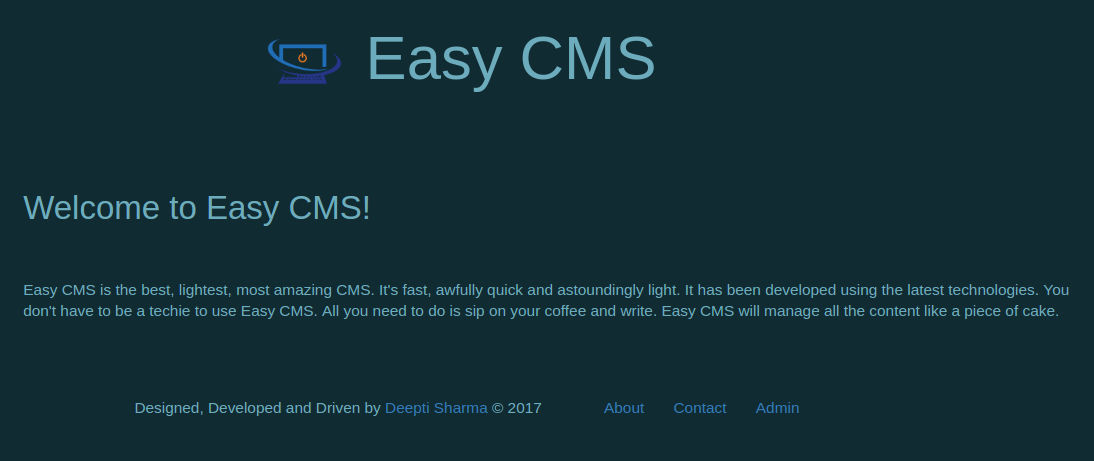
\includegraphics[scale=.45]{input/images/easy1.png}
	\caption{EasyCMS}
\end{figure}

 Easy CMS is the best, lightest, most amazing CMS. It's fast, awfully quick and astoundingly light. It has been developed using the latest technologies. You don't have to be a techie to use Easy CMS. All you need to do is sip on your coffee and write. Easy CMS will manage all the content like a piece of cake..\\
 

 \subsection{Login Panel}

 \begin{figure}[h!]
	\centering 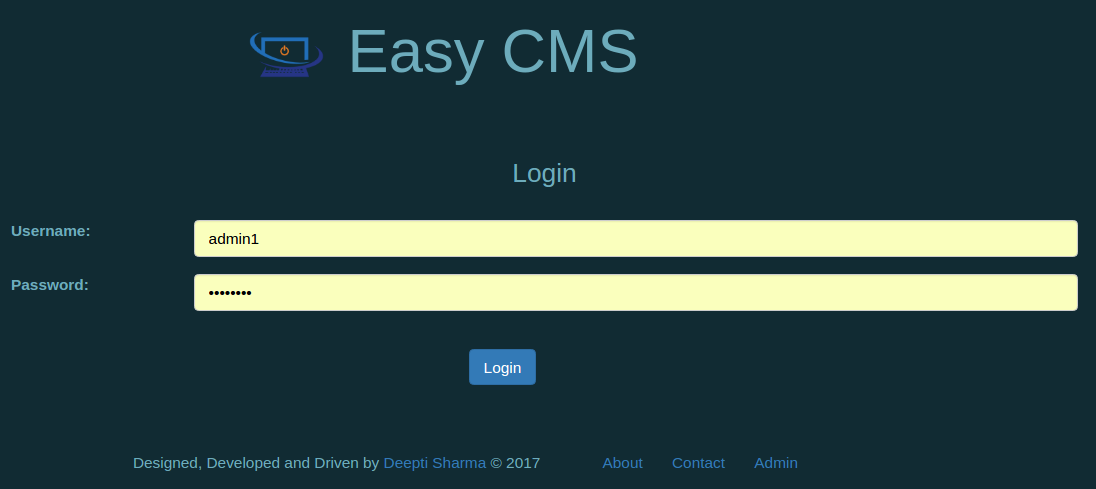
\includegraphics[scale=.45]{input/images/easy2.png}
	\caption{Login}
\end{figure}
This project is completely open source and the entire code is available 
to the user as and when required. There is Complete developer's 
Documentation as well as User manual alongwith it that helps using it a lot easier.\\
Moreover, anyone can use this service and need not have dependencies installed on their systems and can use this service remotely.\\\\

\subsection{Admin Panel}
\begin{figure}[h!]
	\centering 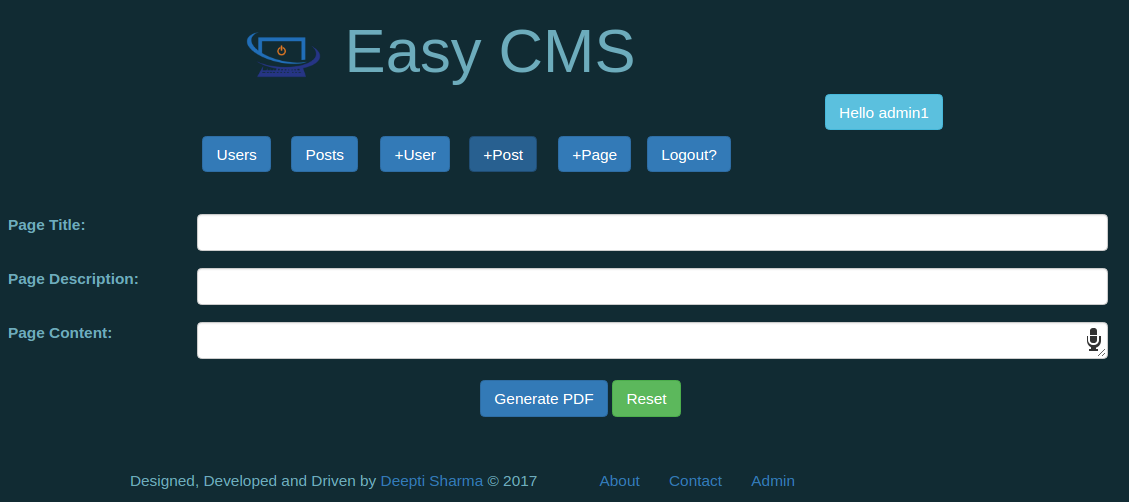
\includegraphics[scale=.45]{input/images/easy3.png}
	\caption{Admin Panel}
\end{figure}

\begin{figure}[h!]
	\centering 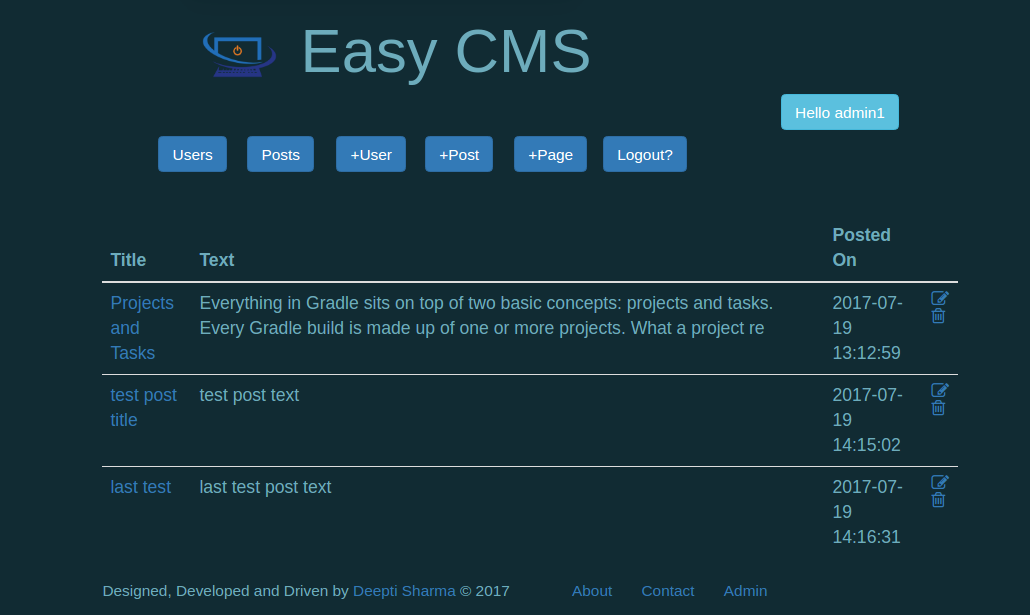
\includegraphics[scale=.49]{input/images/posts.png}
	\caption{Posts}
\end{figure}
Users can create different posts in this and are provided with a secure gateway to login. It provides many features like User creation and speech-recognision which makes it a little different.\\\\
An admin can add users to the CMS and can have a look at the list of active users from the dashboard itself. Admin also acts as a user and can post content and get a PDF document of that.\\
 Even published posts can be displayed under posts section for alteration.
\newpage
\subsection{Generated PDF}
\begin{figure}[h!]
	\centering 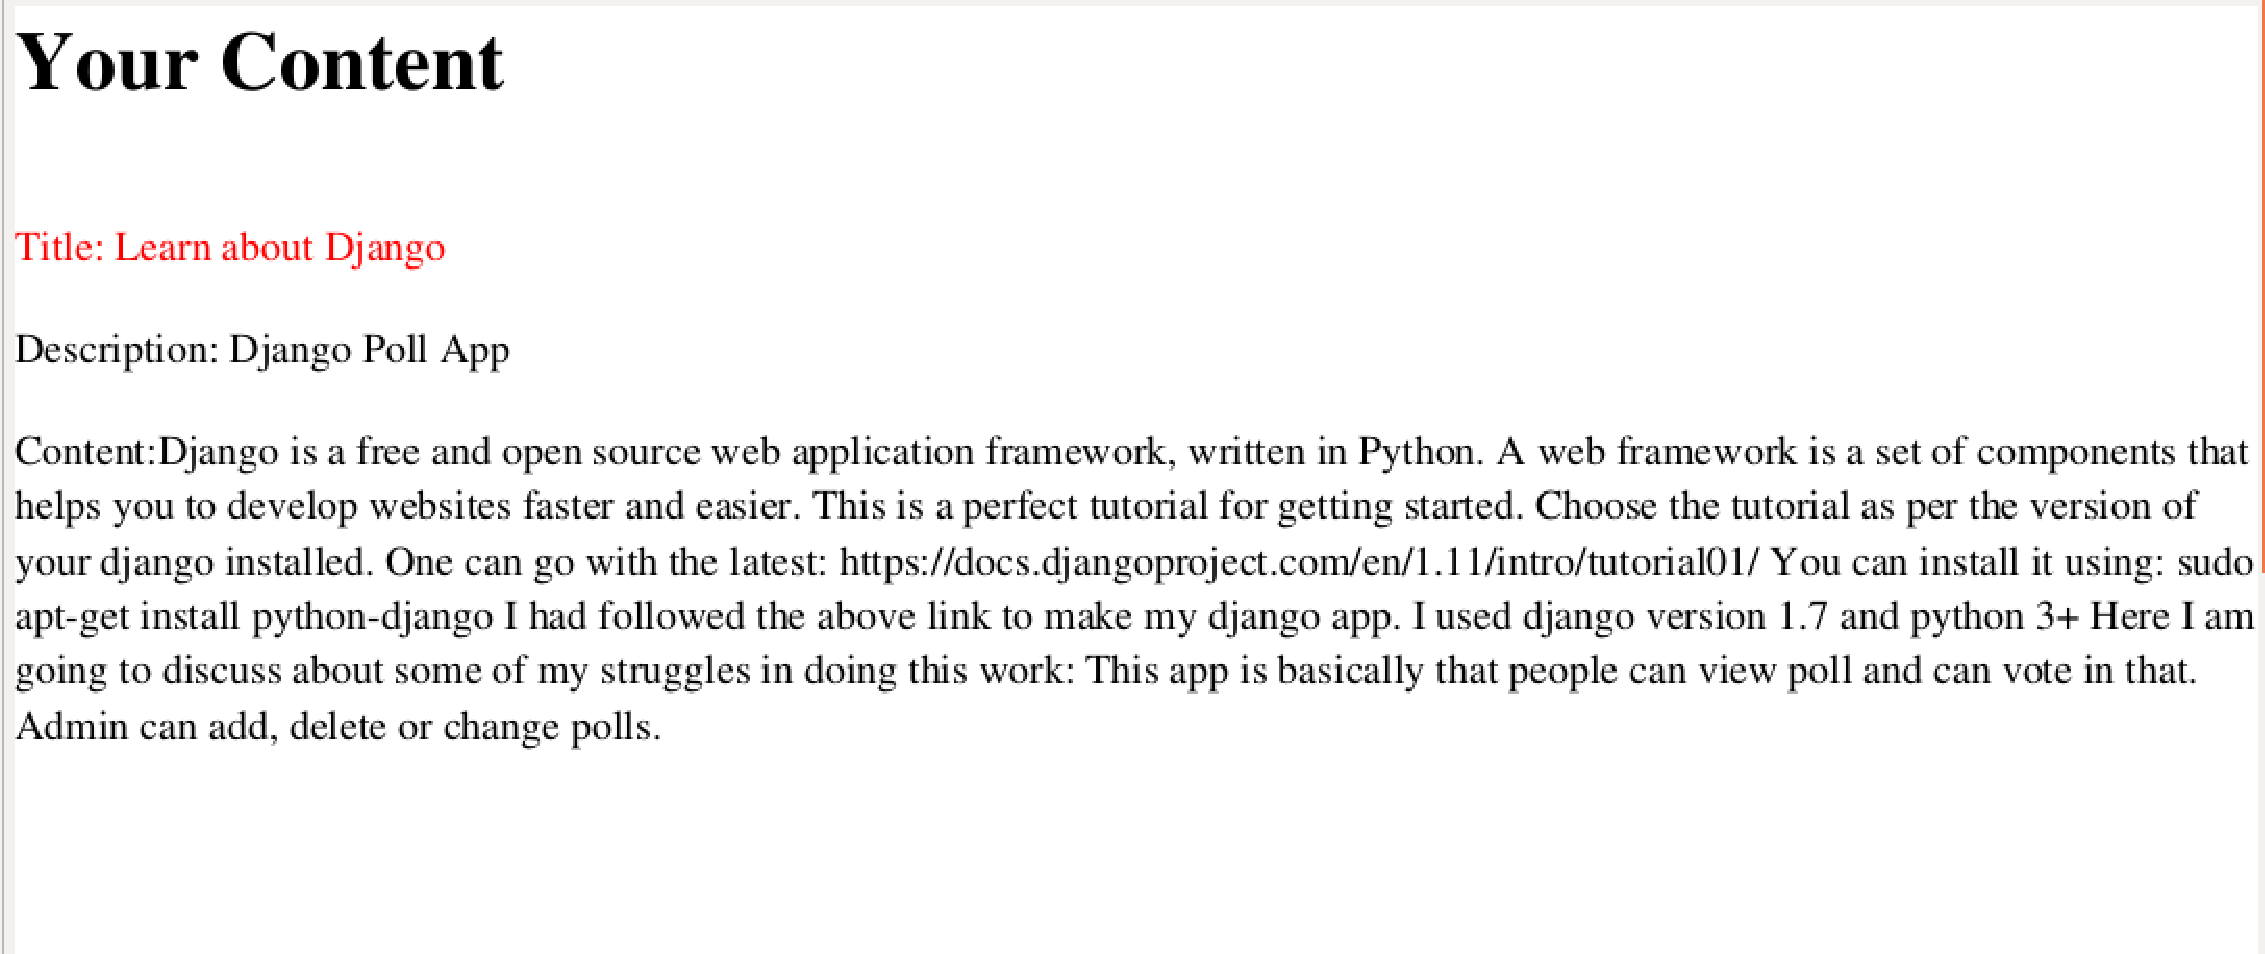
\includegraphics[scale=.47]{input/images/demo.pdf}
	\caption{Sample PDF}
\end{figure}

Using EasyCMS, users can directly take a pdf document of their content saved in the system. It can even be useful to some firms who want to keep a hard copy of some important content or news.


\subsection{Users Control}
\begin{figure}[h!]
	\centering 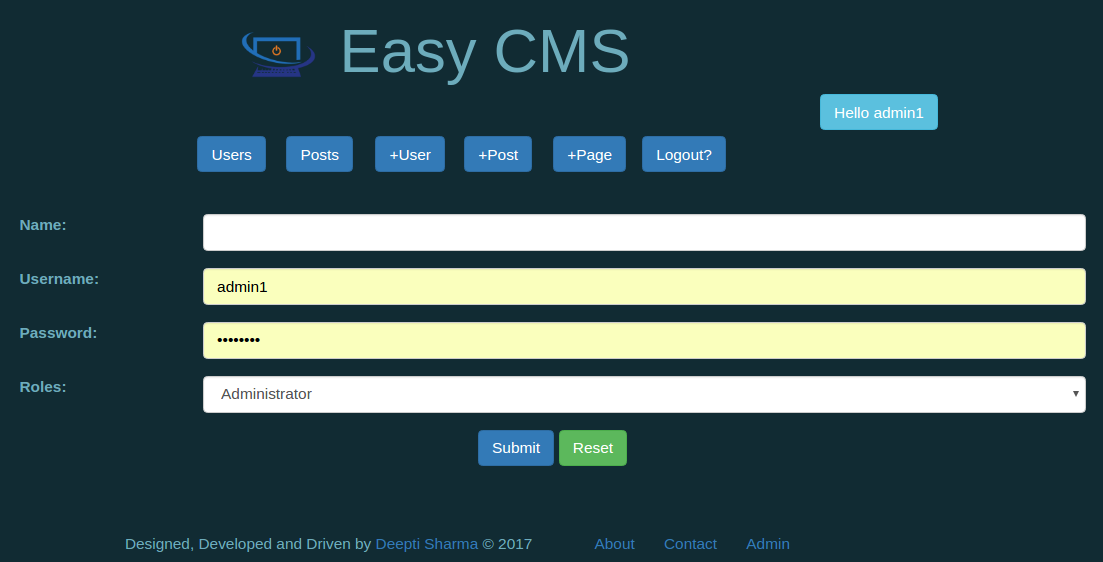
\includegraphics[scale=.45]{input/images/easy4.png}
	\caption{Admin Role}
\end{figure}

Using this feature, CMS can be used in a private firm who want to give access to their employees only.
Only admin can have all these options. Others are there with Addition of posts option only.\\

\begin{figure}[h!]
	\centering 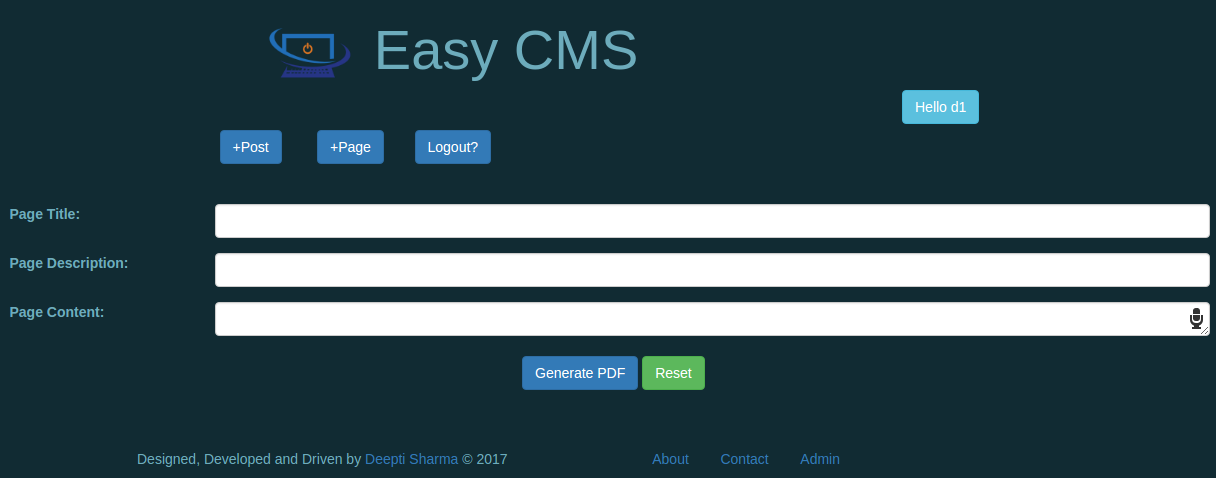
\includegraphics[scale=.40]{input/images/mode.png}
	\caption{Moderator Role}
\end{figure}
\newpage

\begin{figure}[h!]
	\centering 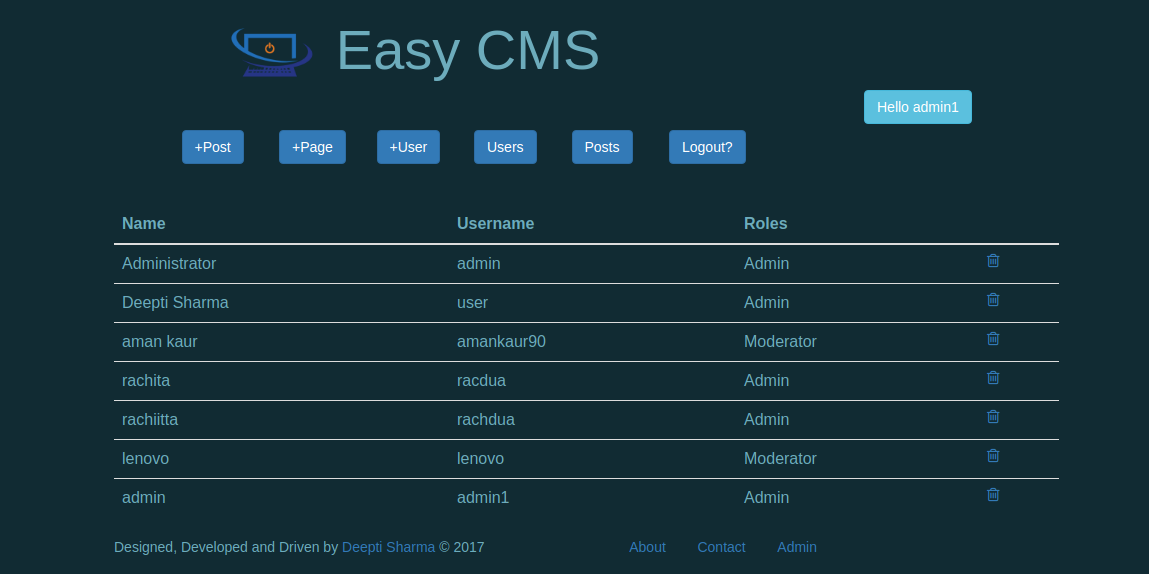
\includegraphics[scale=.42]{input/images/new.png}
	\caption{Users List}
\end{figure}

\subsection{Database}
\begin{figure}[h!]
	\centering 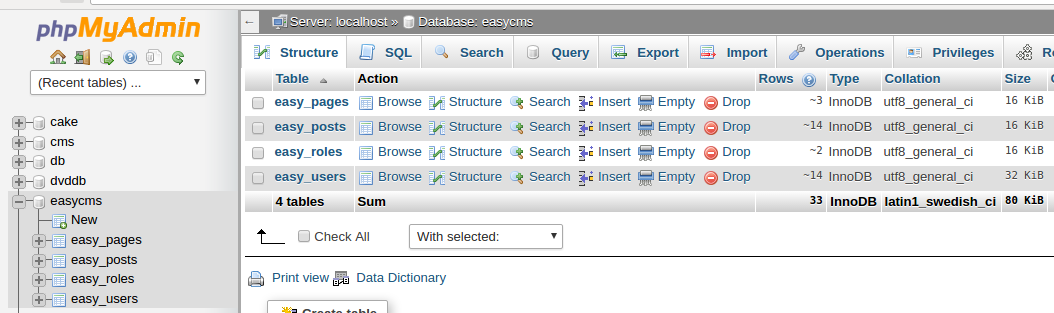
\includegraphics[scale=.45]{input/images/db.png}
	\caption{Database}
	\end{figure}

	MySQL database is used with this project to save the data.
\newpage
 \textbf{GNU/Linux systems:}
 
The working of Content Management System has been checked on various distributions of Linux such as several versions of Ubuntu including 12.04.5 and 14.04.5 (LTS). It was also checked on Fedora and Manjaro. Also a light weight operating system i.e Lubuntu.\\
 
 \textbf{OS X and Windows:}

 This project is operating system independent and will work even on Mac and Windows.\\\\

 
 \textbf{Sources:}
 
Few sources which I considered while building this software are:
\begin{itemize}
\item Quora
\item Online Channels
\item Stack Overflow
\end{itemize}

 \textbf{Installation:}
 Follow the steps below to install EasyCMS:
 \begin{itemize}
 	\item Create a database.
 	\item Access  config/config.php. 
 	\item Enter the database details in the file.
\end{itemize}



 
  
